%\documentclass[referee,usenatbib]{mn2e}
\documentclass[useAMS,usenatbib]{mn2e}

\usepackage{natbib}
\usepackage{graphicx}
\usepackage{url}
\usepackage[utf8]{inputenc}
\usepackage{fancyref}
\usepackage[T1]{fontenc}
\usepackage{array}
\usepackage{rotating}
\usepackage{units}
\usepackage{textcomp}
\usepackage{amsmath}
\usepackage{amsbsy}
\usepackage{amstext}
\usepackage[backref,breaklinks,colorlinks,citecolor=blue]{hyperref}

\newcommand{\msun}{\mbox{$\,{\rm M}_\odot$}}


\title[Gaia Challenge - Palomar 5]{The Gaia Challenge - recovering the galactic potential using a Palomar
5-like stream}

\author[K\"upper et al.]
{Andreas H.W. K\"{u}pper$^{1}$\thanks{
E-mail: \mbox{akuepper@astro.columbia.edu} (AK);
 \mbox{ana.bonaca@yale.edu} (AB);}, Ana Bonaca$^{2}$, Nathan Deg$^{3}$, Adrian Price-Whelan$^{1}$, \newauthor
and so many more\\
$^{1}$Astronomy Department, Columbia University, 550 West 120th Street, New York City, NY 10027, USA\\
$^{2}$Department of Astronomy, Yale University, New Haven, CT 06511, USA\\
$^{3}$Wherever he may be\\
}

\begin{document}

%\date{Accepted 1988 December 15. Received 1988 December 14; in original form 1988 October 11}

%\pagerange{\pageref{firstpage}--\pageref{lastpage}} \pubyear{2002}

\maketitle

\label{firstpage}

\begin{abstract}
\input{abstract.tex}
\end{abstract}




\begin{keywords}
globular clusters --- galactic dynamics
\end{keywords}

\bibliographystyle{mnras}



\section{Introduction}
Tidal streams in the haloes of galaxies are among the most intriguing imprints of hierarchical structure formation in the universe.



\section{The Workshops}
The Gaia Challenge workshop series was initiated in 2013 by Justin Read, Daisuke Kawata and Mark Gieles, and the first meeting was held from 19-23 August 2013 at the University of Surrey in Guildford, England. 
The second edition took place from 27-31 October 2014 at the Max-Planck Institute for Astronomy (MPIA) in Heidelberg, Germany. 
The goal of the workshops is to prepare the modeling community for the vast amount of dynamical data that the Gaia satellite is going to provide us with starting early 2017 \citep{Perryman01}.

Since the richness of the Gaia data will be valuable for a wide range of modeling problems, the workshops are organized in 5 focus groups:
\begin{enumerate}
\item spherical \& triaxial systems,
\item galactic discs,
\item tidal streams \& galactic halo stars,
\item collisional systems
\item astrophysical parameters 
\end{enumerate}
Each of the groups focusses on a different range of problems, each of which is going to benefit from the high expected quality of the Gaia data. For a detailed description of the individual groups, and for an overview of the activities within the groups, see the Gaia Challenge wiki\footnote{\url{http://astrowiki.ph.surrey.ac.uk/dokuwiki/doku.php}}.


\section{The Palomar 5 Challenge}
To generate a Palomar 5-like stream, we ran a direct $N$-body simulation of a low-mass globular cluster, and let it dissolve in a static background potential (see below). The model initially consisted of 65,356 single-mass particles of $0.5\msun$ each, and was evolved for 4\,Gyr using the publicly available code \textsc{Nbody6}. The initial mass of the cluster was $31090\msun$ and it lost $17940\msun$ into the tidal tails, leaving the cluster with a present-day mass of $13150\msun$. The orbit of the cluster was chosen such that the present-day position, distance and radial velocity of the cluster match the observed values for Palomar 5. The position in observable coordinates is $RA = 229.02$\,deg, $Dec = -0.11139$\,deg or $l = 0.85206$\,deg, $b = 45.860$\,deg, its distance was set to $d_{Sun} = 23.2\,pc$ \citep{Harris96}, and the radial velocity was set to -58.7\,km\,s$^{-1}$ \citep{Odenkirchen02}. The proper motion was then chosen such that the profile of the resulting stream matches the observed morphology within the given choice of galactic potential.

With these specifications, the present-day Cartesian coordinates of the progenitor are 
\begin{eqnarray}
  x &=& 7816.082584\,\mbox{pc}\\
  y &=& 240.023507\,\mbox{pc}\\
  z &=& 16640.055966\,\mbox{pc}\\
  vx &=& -37.456858\,\mbox{km\,s}^{-1}\\
  vy &=& -151.794112\,\mbox{km\,s}^{-1}\\
  vz &=& -21.609662\,\mbox{km\,s}^{-1}
\end{eqnarray}

The Challenge can be found on the wiki page of the Gaia Challenge workshop\footnote{\url{http://astrowiki.ph.surrey.ac.uk/dokuwiki/doku.php?id=tests:streams:challenges}}, and we invite everyone to download the Challenge and contribute to this comparison project. The columns are described in the header of the file, and more details can be found on the wiki. The columns give Cartesian coordinates and observables for positions and velocities of all particles. All numbers are either in pc and km/s, or degree and mas/yr, respectively. 

The Cartesian coordinates are given in the Galactic rest frame. The observables were derived assuming a solar Galactocentric distance of 8.33\,kpc and a LSR motion of 239.5\,km/s \citep{Gillessen09}. In addition, the solar reflex motion was assumed to be $(11.1, 12.24, 7.25)$\,km\,s$^{-1}$ \citep{Schonrich10}.  





\subsection{The potential}

The functional form of the potential components is as follows:

Flattened NFW halo:

\begin{eqnarray}
  \Phi_{Halo}(R, z) &=& -\frac{GM}{\sqrt{R^2+\frac{z^2}{q_z^2}}}\ln\left(1+\frac{\sqrt{R^2+\frac{z^2}{q_z^2}}}{R_{Halo}} \right)\\
  M_{Halo} &=& 1.81194\times 10^{12}\msun\\
  R_{Halo} &=& 32260\,pc\\
  q_z &=& 0.8140
\end{eqnarray}

Jaffe bulge:

\begin{eqnarray}
  \Phi_{Bulge} &=& \frac{GM_{Bulge}}{b_{bulge}}\ln{\frac{R}{R+b_{bulge}}}\\
  M_{Bulge} &=& 3.4\times 10^{10}\msun\\
  b_{Bulge} &=& 700.0\,\mbox{pc}
\end{eqnarray}

Miyamoto-Nagai disk:
\begin{eqnarray}
  \Phi_{Disk} &=& -\frac{GM_{Disk}}{\sqrt{R^2+\left(a_{Disk}+\sqrt{z^2+b_{Disk}^2}\right)^2}}\\
  M_{Disk} &=& 1.0\times 10^{11}\,M_{\odot}\\
  a_{Disk} &=& 6500\,pc\\
  b_{Disk} &=& 260\,pc
\end{eqnarray}

\begin{itemize}
  \item $V_C(R_{Sun}) = 249.01\,km/s$
  \item $V_C(R_{Pal5}) = 247.84\,km/s$
  \item $V_C(R_{Halo}) = 251.99\,km/s$
  \item $a(R_{Sun}, 0, 0) = 7.95\,pc/Myr^2$
  \item $a(R_{Pal5}) = a(7816 pc, 240 pc, 16640 pc) = 3.51\,pc/Myr^2$
  \item $a(R_{Halo}, 0, 0) = 2.06\,pc/Myr^2$
\end{itemize}





\section{The Methods}
Quite interesting text about the methods.

\subsection{Ana Bonaca}
For the \textsc{FastForward} method, forward models of streams are generated using the streakline method outlined in \citet{Kupper12} and \citet{Bonaca14}. 
Starting from the present-day position of the cluster, its orbit is integrated backwards in a given trial galaxy potential for a specified time. 
In the case of this test problem, the 3D position and velocity of the cluster is known as well as the integration time of the underlying $N$-body model. 
Hence, these parameters are fixed and only the parameters of the halo potential are sampled from a parameter probablity distribution using the Markov-chain Monte Carlo sampler \textit{emcee} \citep{Foreman13}.

From these initial conditions, the cluster is integrated back to the present-day position, while test particles are released from the instantaneous Lagrange points of the cluster-galaxy system at fixed time intervals of 40\,Myr, resulting in 100 test particles per stream (leading/trailing). 
The positions of the Lagrange points are calculated using the approximation for the Jacobi radius from \citet{King62},
\begin{equation}
r_{L} = \left( \frac{G\,M_c}{\Omega_c^2-\partial^2\Phi/\partial R_c^2}\right)^{1/3},
\end{equation}
where $G$ is the gravitational constant, $M_c$ is the mass of the cluster, $\Omega_c$ is the instantaneous angular velocity of the cluster, and $\partial^2\Phi/\partial R_c^2$ is the second derivative of the galactic potential with respect to the cluster's galactocentric radius, $R_c$.
Test particles are released from $\pm r_L$ along the connecting line between cluster center and galactic center with velocities matching the cluster's angular velocity. 
Random spacial and velocity offsets from these idealized escape conditions are added to the test particles. 
They are drawn from gaussian distributions with dispersions of $0.25r_L$ and 1\,km\,s$^{-1}$, respectively.
 
The resulting, present-day positions and velocities of stream test particles,  are then compared to the mock model particles using a likelihood function of the form
\begin{equation}
L = \prod_j^{N_{data}} \left(\frac{1}{N_{model}}\sum_i^{N_{model}} \exp{\left(-\frac{d_{ij}^2}{2\Delta d^2}\right)} \right).
\end{equation} 
Here, $N_{data}$ is the number of data points of the mock model, $N_{model}$ is the number of model points from the forward model, $d_{ij}$ is the distance of the $i$-th model point from the $j$-th data point in 6D-phase space, and $\Delta d$ is the uncertainty in this distance. 
Since the given data is error-free, hyper-parameters are used to artificially widen the distribution of the points, and create a continuos density distribution. 
This likelihood value is then used as input for the MCMC sampler. 
The chains presented here are the results of 64 ``walkers'', making a total of 200 steps each, after a short burn-in phase of 20 steps.


\subsection{Jo Bovy}
Some details on the method: I fit 200 points without errors (but effectively assuming that the errors are smaller than the width of the stream, because I use an estimated width of the stream in comparing model vs. data) and the likelihood is just the best-fit orbit's likelihood for each trial potential (I don't marginalize over the orbit for each potential).


\subsection{Nathan Deg}

The orbit-fitting method assumes that the stream is generated by the orbit of a single particle in a fixed potential.  
Due to this method's simplicity, it is the most efficient stream modelling method.  We use a modified version of the 
algorithm described in \citet{Deg13}.  The main difference is that the likelihood is calculated for a data point being drawn 
from the entire \textit{stream} rather than from the nearest stream point.  Explicitly, the likelihood of particular 
data point, $D_{j}$ being drawn from a model stream, $\mathbf{M}$, is
is 
\begin{equation}
 \mathcal{L}(D_{j}|\mathbf{M})=\sum_{i=1}^{N}\mathcal{L}(D_{j}|M_{i})~,
\end{equation}
where $N$ is the number of points comprising the stream and $M_{i}$ is the $i$-th orbital point. The likelihood of being 
drawn from each model stream point is  
\begin{equation}
 \mathcal{L}(D_{j}|M_{i})=\Pi_{k}^{N_{k}}\frac{1}{\sqrt{2\pi\sigma_{k}^{2}}}
 e^{-\frac{(D_{j,k}-M_{i,k})^{2}}{2\sigma_{k}^{2}}}~,
\end{equation}
where $N_{k}$ is the number of phase-space observations of the data point, and $\sigma_{k}$ is the combined error and thickness 
associated with that phase-space observation.  Any stream has some thickness or dispersion in each dimension and every observation 
has some error.  In this test case we do not include any observational error but we do fit for a uniform thickness in each dimension.
This introduces a number of additional free parameters.

For simplicity we model the MW using the generative Jaffe bulge, Miyamoto-Nagai disk, and flattened NFW halo with 
all parameters fixed except the halo mass, scale length, and flattening.  To recover the PDF, we performed a Bayesian analysis with logarithmic priors on all 
MW model free parameters using the \textit{emcee} algorithm with 200 walkers each run for 2000 steps.


\subsection{Kohei Hattori}
We use the variation of kinetic energy of stream particles along the stream, which can be interpreted as the variation of gravitational potential. We can determine the flattening of the potential if the kinetic energy does not monotonically increase or decrease along the stream.

I use 50 randomly selected stars (without error) from the leading or trailing streams. I assumed the correct parameters for disc and bulge potential as well as the correct scale length for the halo potential. I model the orbital energy distribution in each tail as a Gaussian distribution and run an emcee code to derive the posterior distribution of $(M/(10^{12}\msun), q_z)$.

\subsection{Sergey Koposov}
Orbit fits. Only trailing tail was used. ``Realistic'' errors have been assumed. ~ 1-2 km/s RV precision ~1\% distance errors, 0.1-0.2 mas/yr. The potential was a Miyamoto-Nagai disk + bulge + NFW halo with narrow Gaussian priors on everything except the halo.

\subsection{Adrian Price-Whelan}
I use 4 stars randomly drawn from the tails of the simulated Pal 5 stream to fit for the halo parameters, with fixed bulge and disk parameters. This is a trivial test because I use the same potential to fit as the simulation was run in, I fix the disk and bulge, and I am using perfect data. Here is the marginal posterior over just the halo potential parameters (marginalizing over nuisance parameters I use to model the debris).

\subsection{Jason Sanders}
Construct a model for a single stream by using information about the form of the stream in angle-frequency space in the true potential. The model favours two narrow clumps in frequency space aligned with the angle structure.

I attempted to fit the potential with the location of the progenitor known and no errors. I used only 30 stars. I fitted both a logarithmic potential (just two parameters circular velocity Vc and flattening q) and the full potential used for the simulation with all parameters bar the halo parameters held fixed.


\section{Results}
Many interesting results.

\subsection{Ana Bonaca}\label{ssec:ana_results}
\begin{figure}
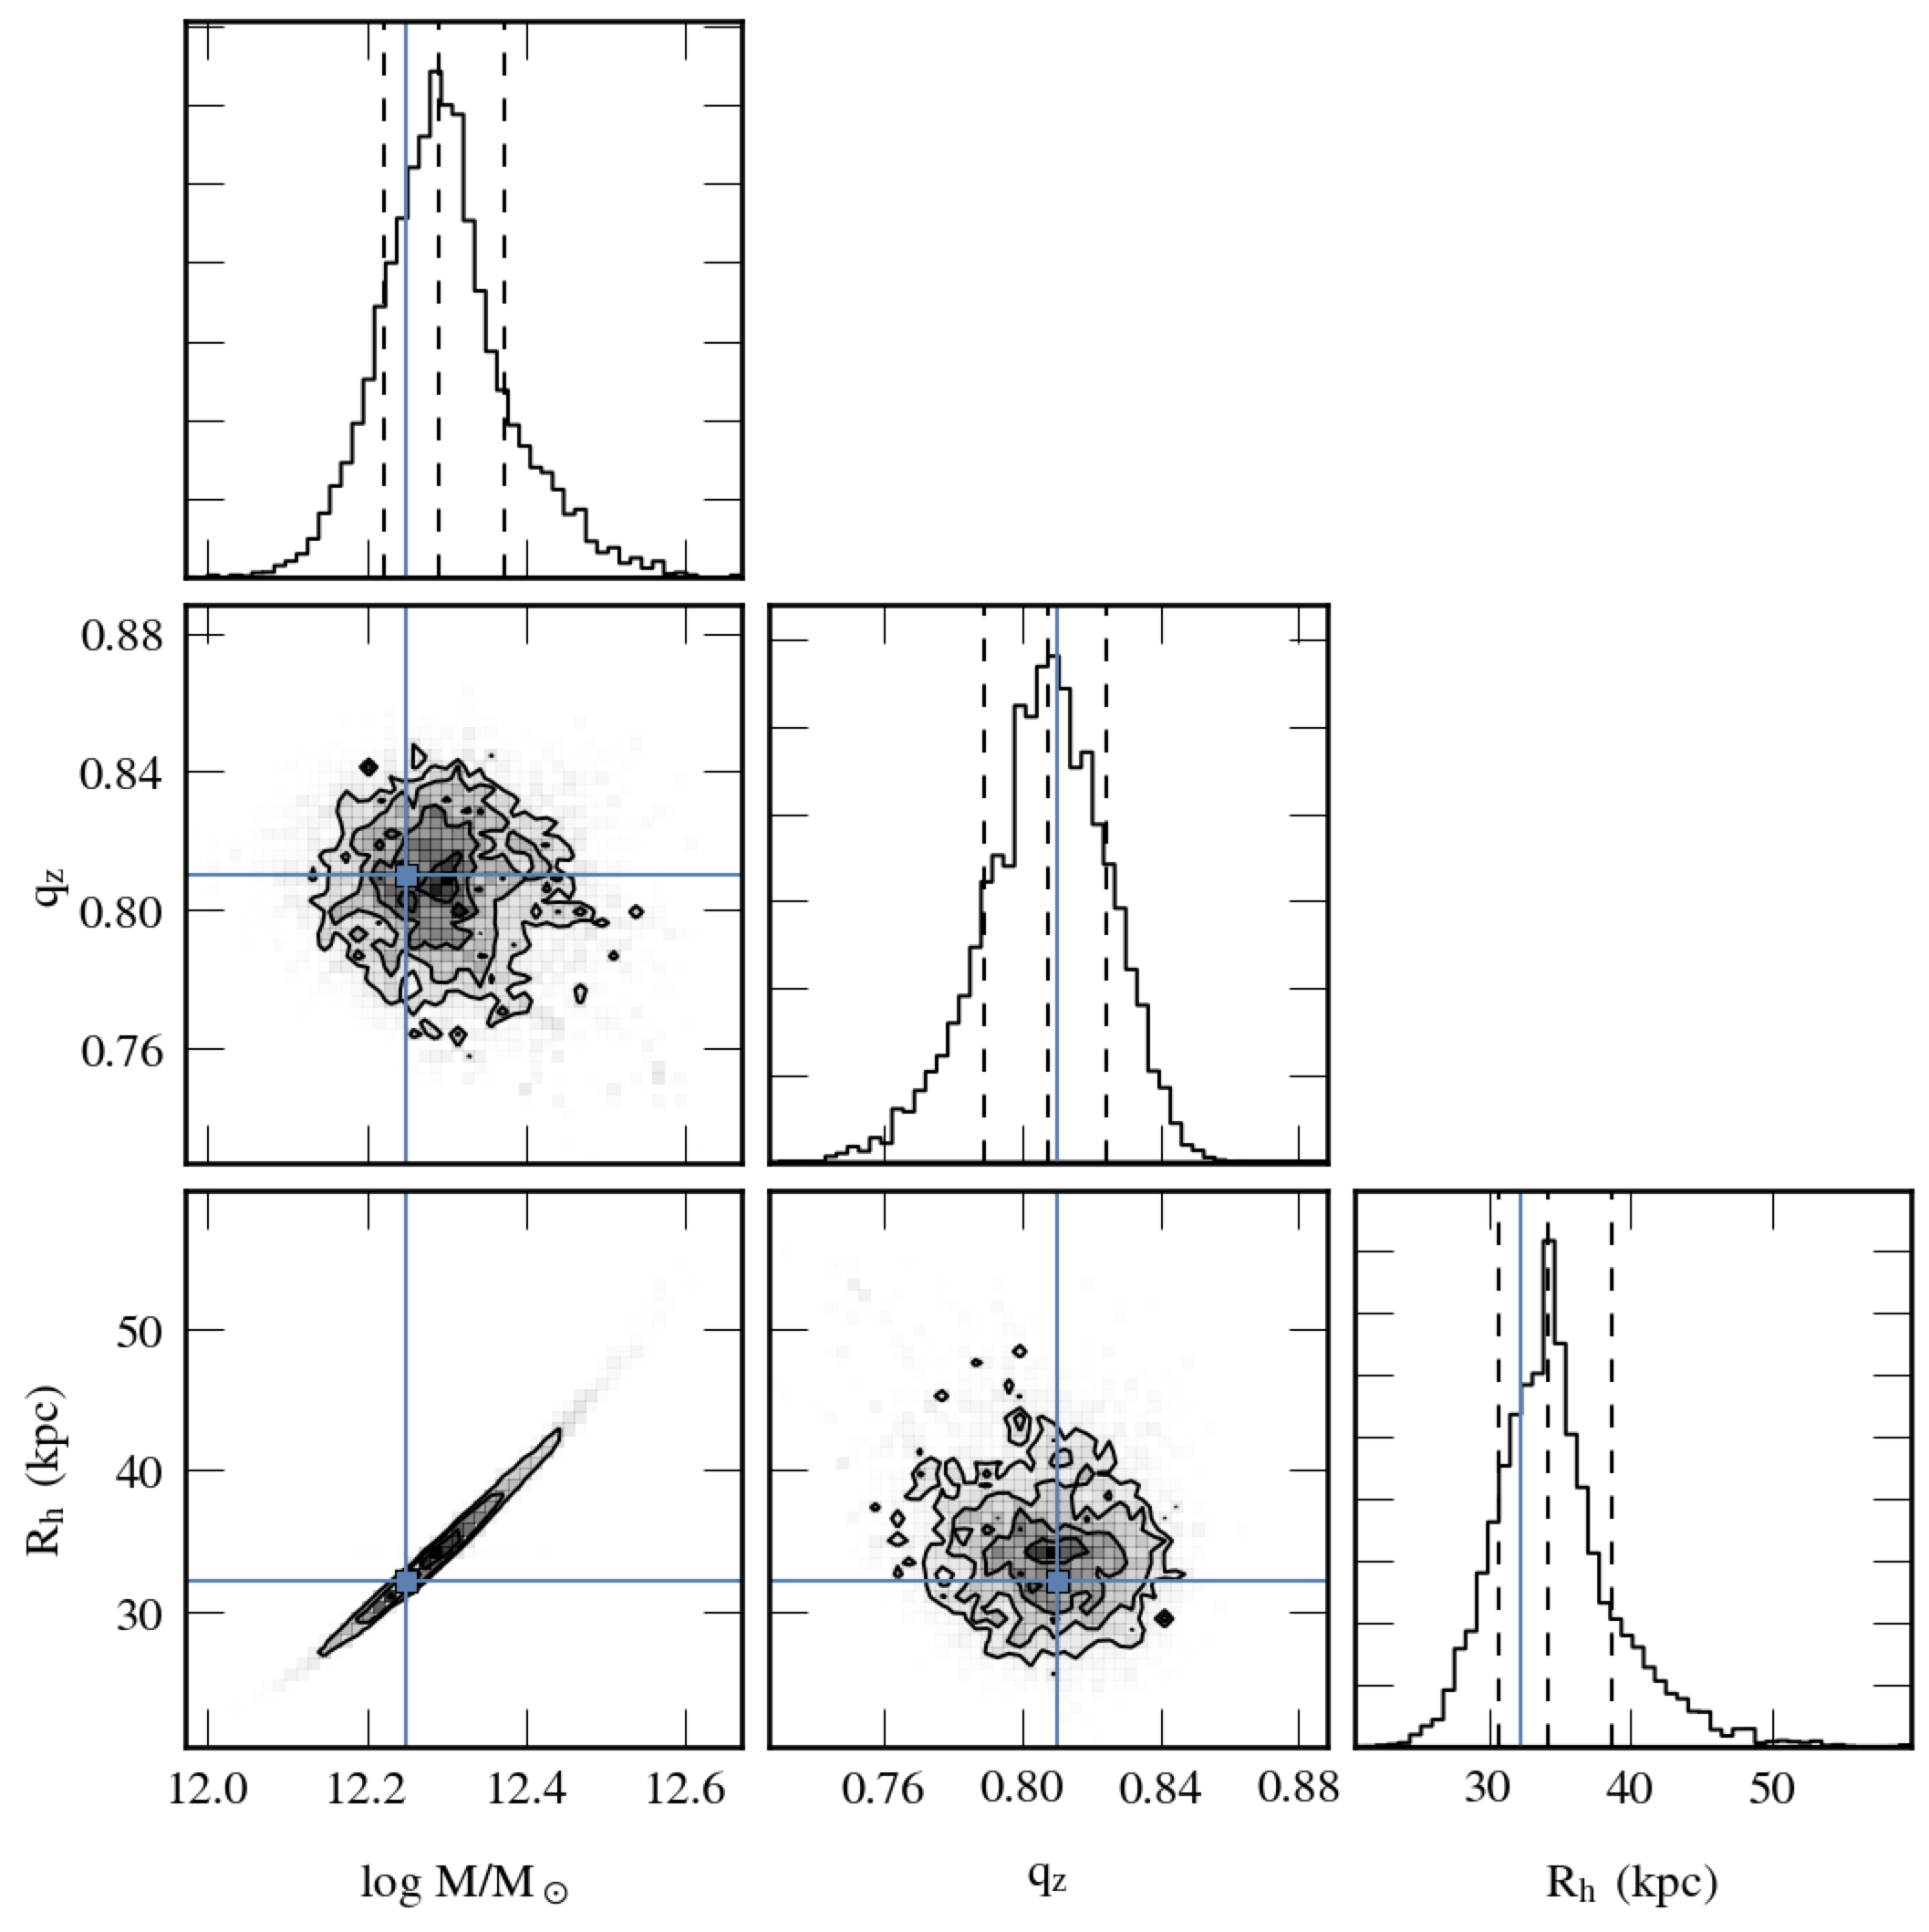
\includegraphics[width=83mm]{./figures/ana_results.png}
  \caption{Ana's results (Sec.~\ref{ssec:ana_results})}
  \label{plot_ana_results}
\end{figure}

For Ana's results see Fig.~\ref{plot_ana_results}.


\subsection{Jo Bovy}\label{ssec:jo_results}
\begin{figure}
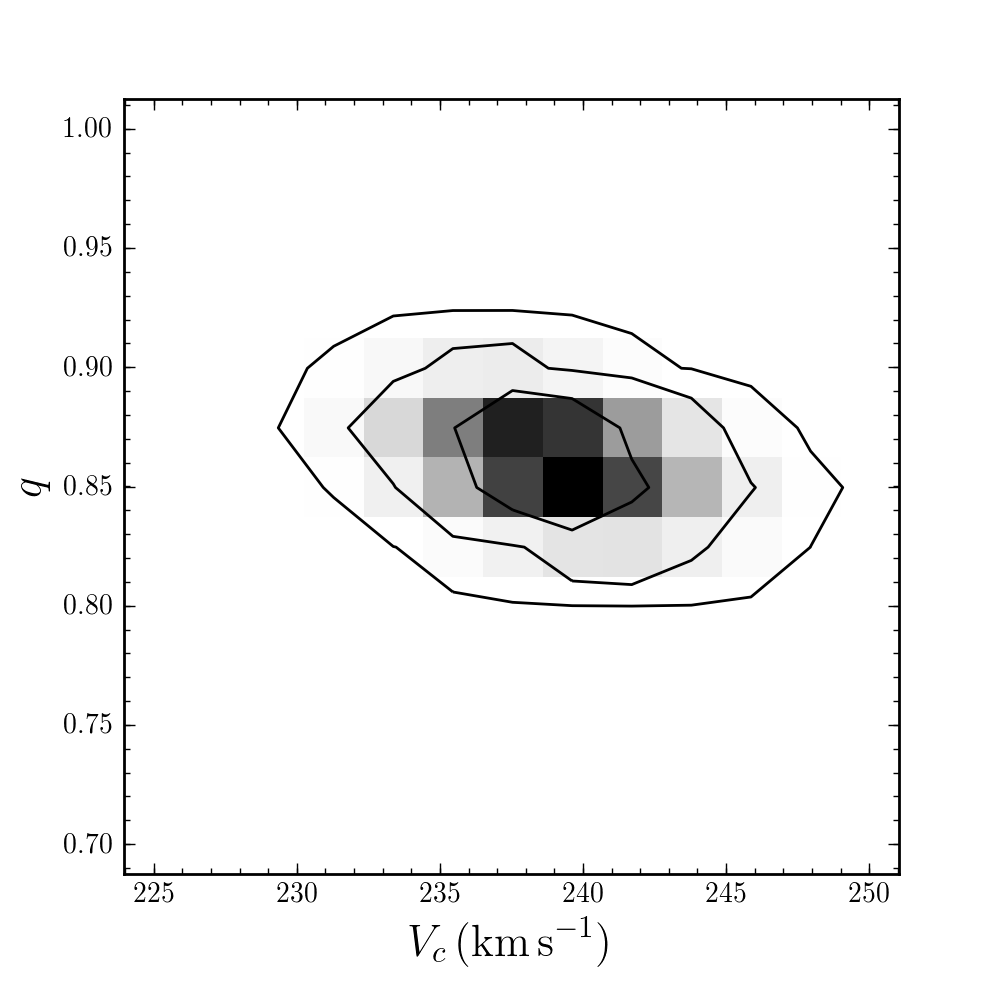
\includegraphics[width=83mm]{./figures/jo_results.png}
  \caption{Jo's results (Sec.~\ref{ssec:jo_results})}
  \label{plot_jo_results}
\end{figure}

\begin{figure}
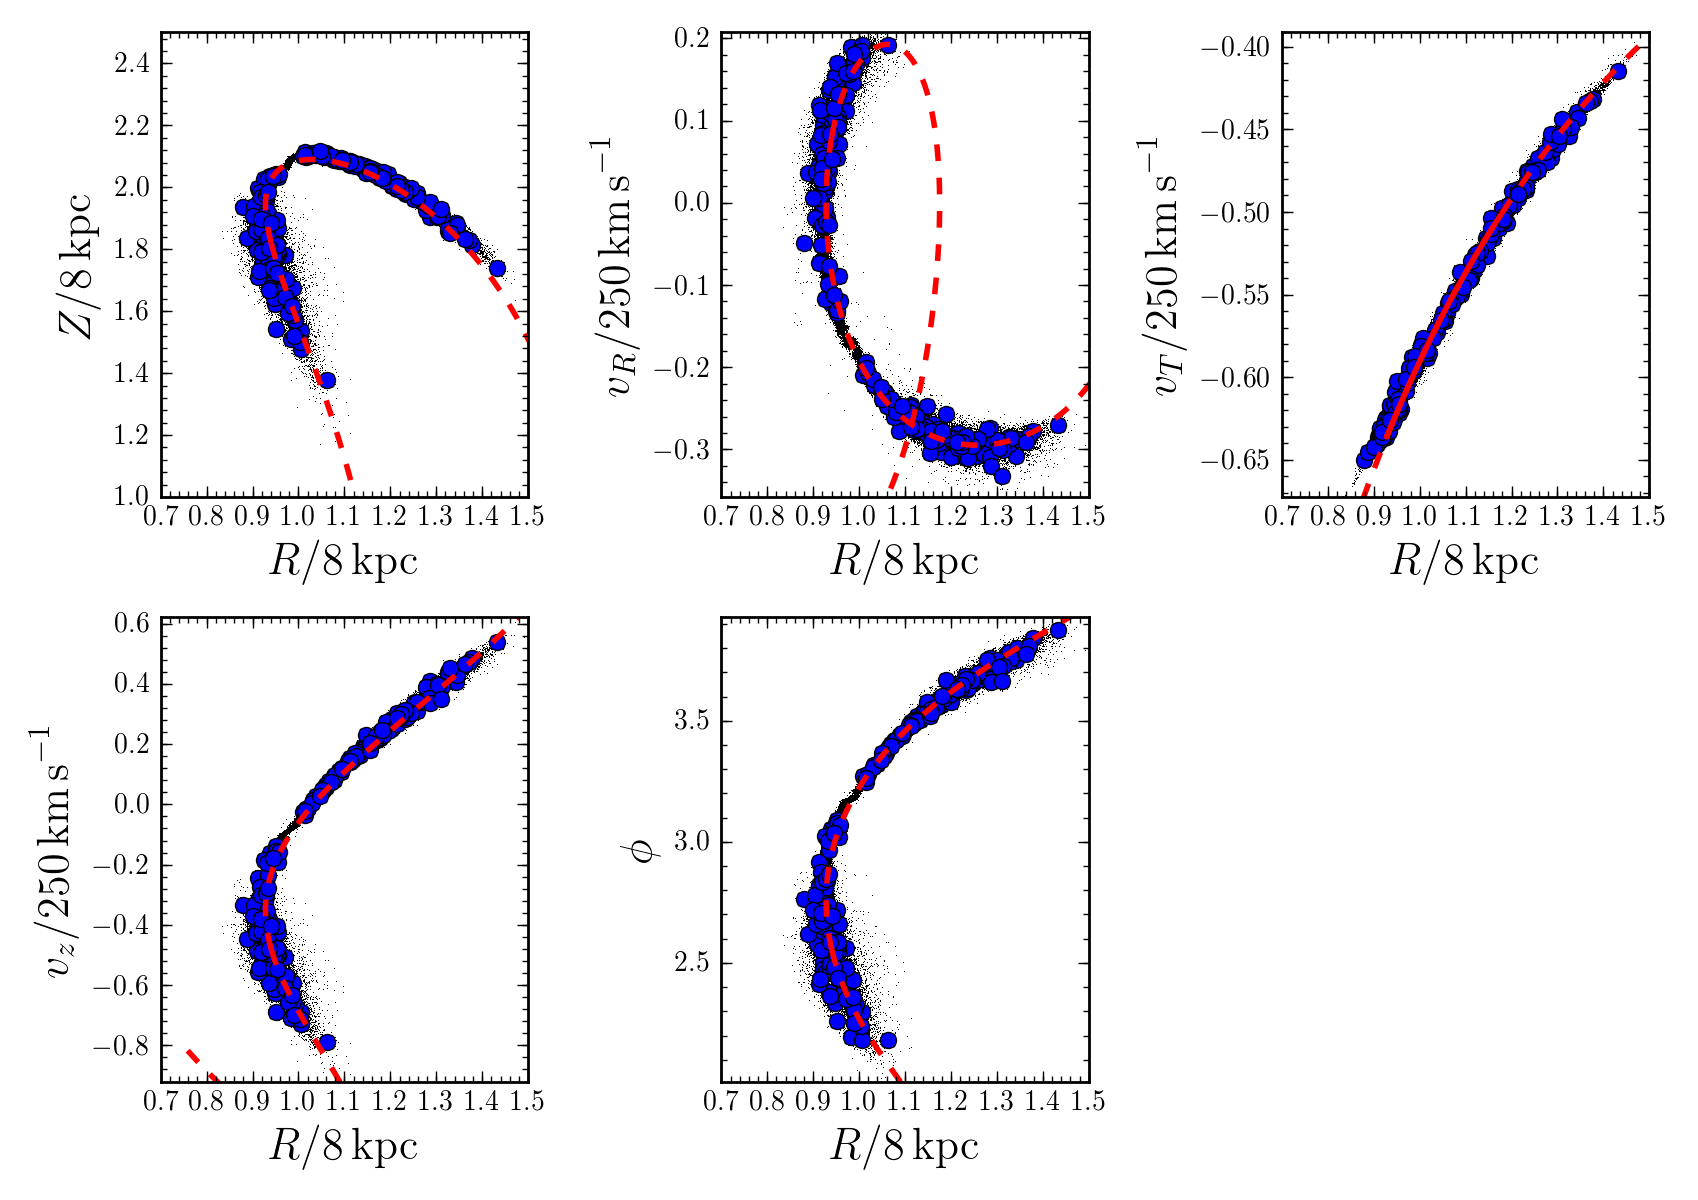
\includegraphics[width=83mm]{./figures/jo_orbitfit.png}
  \caption{Jo's results (Sec.~\ref{ssec:jo_results})}
  \label{plot_jo_orbitfit}
\end{figure}

I computed the acceleration at Pal 5 and get
$a(Pal5) = 3.42 \pm 0.04 pc/Myr^2$.

The PDF in Fig.~\ref{plot_jo_results} shows 1, 2, and 3 sigma contours. 
I just fit a flattened logarithmic potential, so the PDF is for those two parameters ($v_c$ and flattening $q$). 
The orbit fit in Fig.~\ref{plot_jo_orbitfit} shows different projections: I fit to the 200 blue points, the best-fitting orbit is shown in red.


\subsection{Nathan Deg}\label{ssec:nathan_results}
To test the basic orbit-fitting algorithm we used 100 points randomly selected from the stream and fit their 
Cartesian coordinates.  In Cartesian space, each data point consists of six phase-space observations.  This means 
that we fit six thickness parameters for a total of nine free parameters.  The resulting MW model PDFs are shown in 
Fig. \ref{plot_nathan_results_Cart}.  The halo flattening is recovered within the 68\% confidence limits, but the orbit
fitting algorithm only recovers the correlation between the  halo mass and scale radius.  The degeneracy in these 
two parameters is due to the orbit-fitting method only being sensitive to the mass within the orbit.  In an NFW halo, 
all models within the mass-radius band indicated in Fig. \ref{plot_nathan_results_Cart} have the same 
mass within the Pal 5 orbit and, as shown in Fig. \ref{plot_nathan_results_Cart_accel}, give the same acceleration at the location 
of the Pal 5 progenitor.  However, this figure also demonstrates that the orbit-fitting algorithm does not quite 
recover the true model as the inferred acceleration differs from the true acceleration significantly.

\begin{figure}
\includegraphics[width=83mm]{./figures/Nathan_results_CartAll.pdf}
  \caption{The MW model PDFs inferred using the orbit-fitting algorithm on Cartesian stream data.  The red and blue 
  contours enclose the 68\% and 95\% confidence regions, the star and red vertical lines indicate 
  the generative values, and the grey shaded regions correspond to areas of increasing 
  probability.  (Sec.~\ref{ssec:nathan_results})}
  \label{plot_nathan_results_Cart}
\end{figure}

\begin{figure}
\includegraphics[width=83mm]{./figures/Nathan_results_Accel_CartAll.pdf}
  \caption{The inferred acceleration at the location of the Pal-5 progenitor using the 
  orbit-fitting algorithm with Cartesian data.  The red line indicates the generative value.  (Sec.~\ref{ssec:nathan_results})}
  \label{plot_nathan_results_Cart_accel}
\end{figure}


A slightly more realistic test is to utilize observational data instead of Cartesian data.  Observational data differs from Cartesian 
data in two key respects.  Firstly, it reduces the dimensionality of the stream fitting to five phase-space coordinates as 
we use the angular distance on the sky between model stream points and data points as the constraint.  Secondly, it introduces 
a constraint on the local circular speed as the observations of the stream's radial velocity and proper motions are 
convolved with $v_{c}(R_{\circ})$.  The resulting PDFs of the model parameters and acceleration at the location of the 
Pal 5 progenitor are shown in Figs. \ref{plot_nathan_results_ObsData}-\ref{plot_nathan_results_ObsData_accel}.
These figures show that the use of observational data improves the fits greatly.  The convolution of the observed
motion with the local circular speed breaks the halo mass-scale radius degeneracy.  The generative model is recovered, as 
is the acceleration at the location of Pal 5.


\begin{figure}
\includegraphics[width=83mm]{./figures/Nathan_results_ObsData.pdf}
  \caption{The MW model PDFs inferred using the orbit-fitting algorithm on Cartesian stream data.  The red and blue 
  contours enclose the 68\% and 95\% confidence regions, the star and red vertical lines indicate 
  the generative values, and the grey shaded regions correspond to areas of increasing 
  probability.  (Sec.~\ref{ssec:nathan_results})}
  \label{plot_nathan_results_ObsData}
\end{figure}

\begin{figure}
\includegraphics[width=83mm]{./figures/Nathan_results_Accel_ObsData.pdf}
  \caption{The inferred acceleration at the location of the Pal-5 progenitor using the 
  orbit-fitting algorithm with Cartesian data.  The red line indicates the generative value.  (Sec.~\ref{ssec:nathan_results})}
  \label{plot_nathan_results_ObsData_accel}
\end{figure}

It is worth noting that these tests are still not completely realistic.  The progenitor has remained fixed in Cartesian space, no 
observational error has been included, and the majority of the model parameters were not explored.  While the results shown in 
Figs. \ref{plot_nathan_results_ObsData}-\ref{plot_nathan_results_ObsData_accel} are promising, it is not clear how well 
orbit-fitting will perform in more realistic tests.

\subsection{Kohei Hattori}\label{ssec:kohei_results}
\begin{figure}
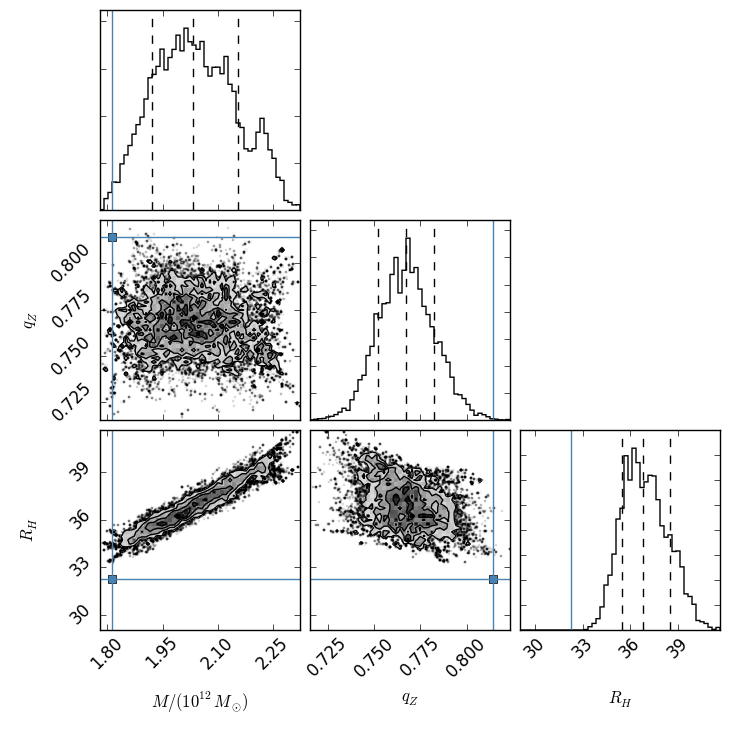
\includegraphics[width=83mm]{figures/kohei_results1.png}
  \caption{Kohei's results (Sec.~\ref{ssec:kohei_results})}
  \label{plot_kohei_results1}
\end{figure}

\begin{figure}
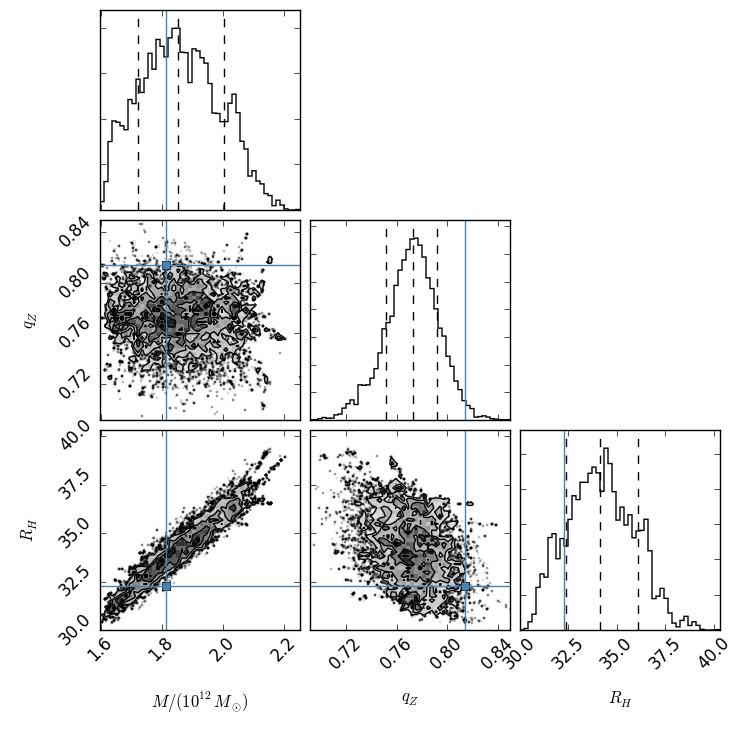
\includegraphics[width=83mm]{figures/kohei_results2.png}
  \caption{Kohei's results (Sec.~\ref{ssec:kohei_results})}
  \label{plot_kohei_results2}
\end{figure}

\begin{figure}
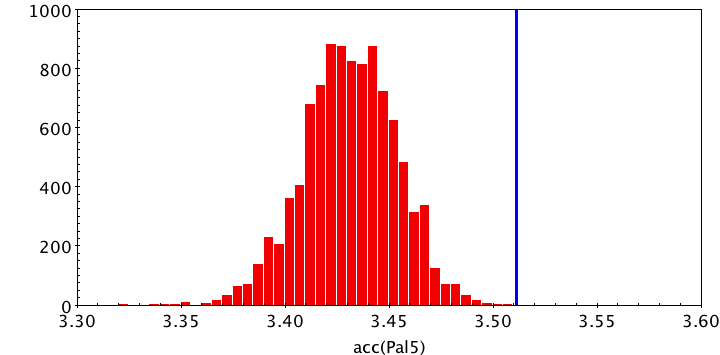
\includegraphics[width=83mm]{figures/kohei_acc.png}
  \caption{Kohei's results (Sec.~\ref{ssec:kohei_results})}
  \label{plot_kohei_acc}
\end{figure}

Kohei's results are in Figs.~\ref{plot_kohei_results1}, \ref{plot_kohei_results2} and ~\ref{plot_kohei_acc}.


\subsection{Sergey Koposov}\label{ssec:sergey_results}
\begin{figure}
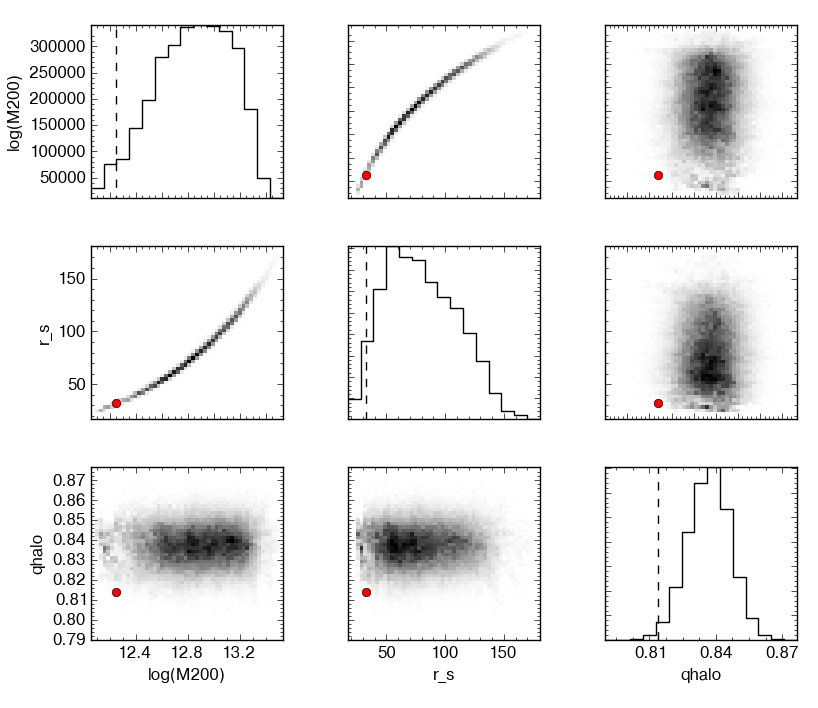
\includegraphics[width=83mm]{./figures/sergey_results.png}
  \caption{Sergey's results (Sec.~\ref{ssec:sergey_results})}
  \label{plot_sergey_results}
\end{figure}

\begin{figure}
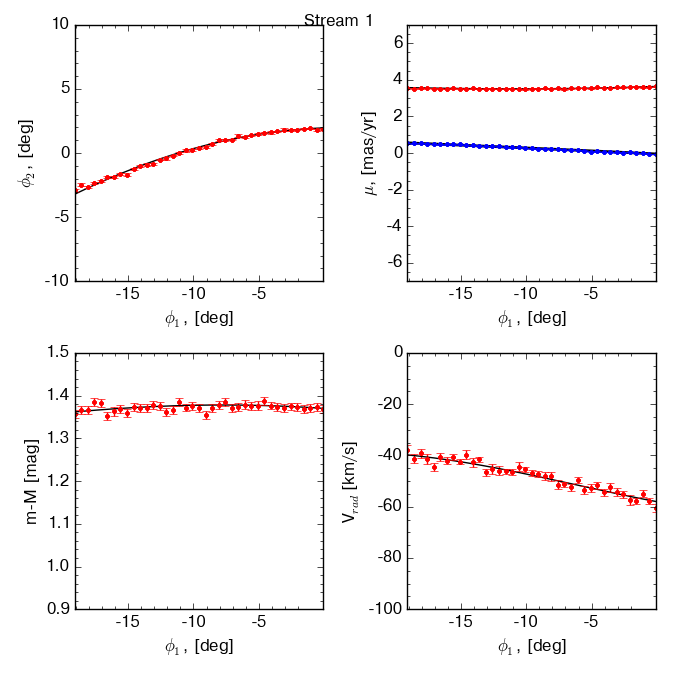
\includegraphics[width=83mm]{./figures/sergey_orbitfit.png}
  \caption{Sergey's results (Sec.~\ref{ssec:sergey_results})}
  \label{plot_sergey_orbitfit}
\end{figure}

\begin{figure}
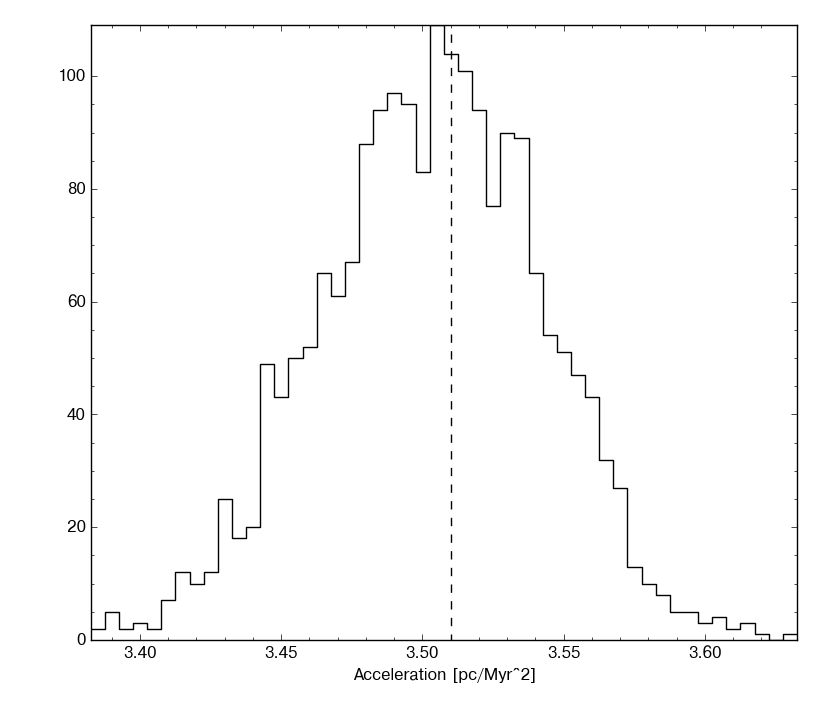
\includegraphics[width=83mm]{./figures/sergey_acc.png}
  \caption{Sergey's results (Sec.~\ref{ssec:sergey_results})}
  \label{plot_sergey_acc}
\end{figure}

The acceleration at Pal5 is $3.50 \pm 0.03 pc/Myr^2$ (Fig.~\ref{plot_sergey_acc}).



\subsection{Jorge Pe\~narrubia}\label{ssec:jorge_results}
\begin{figure}
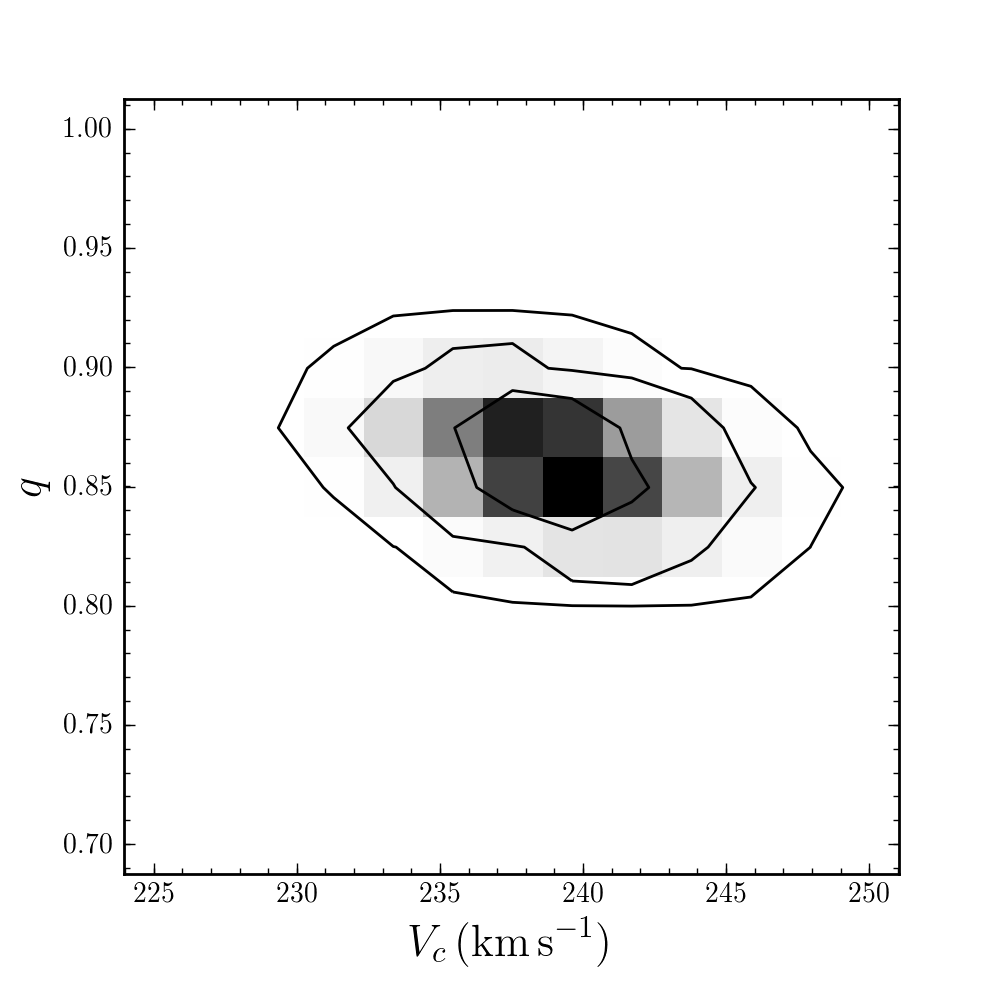
\includegraphics[width=83mm]{./figures/jo_results.png}
  \caption{Jo's results (Sec.~\ref{ssec:jo_results})}
  \label{plot_jo_results}
\end{figure}

\begin{figure}
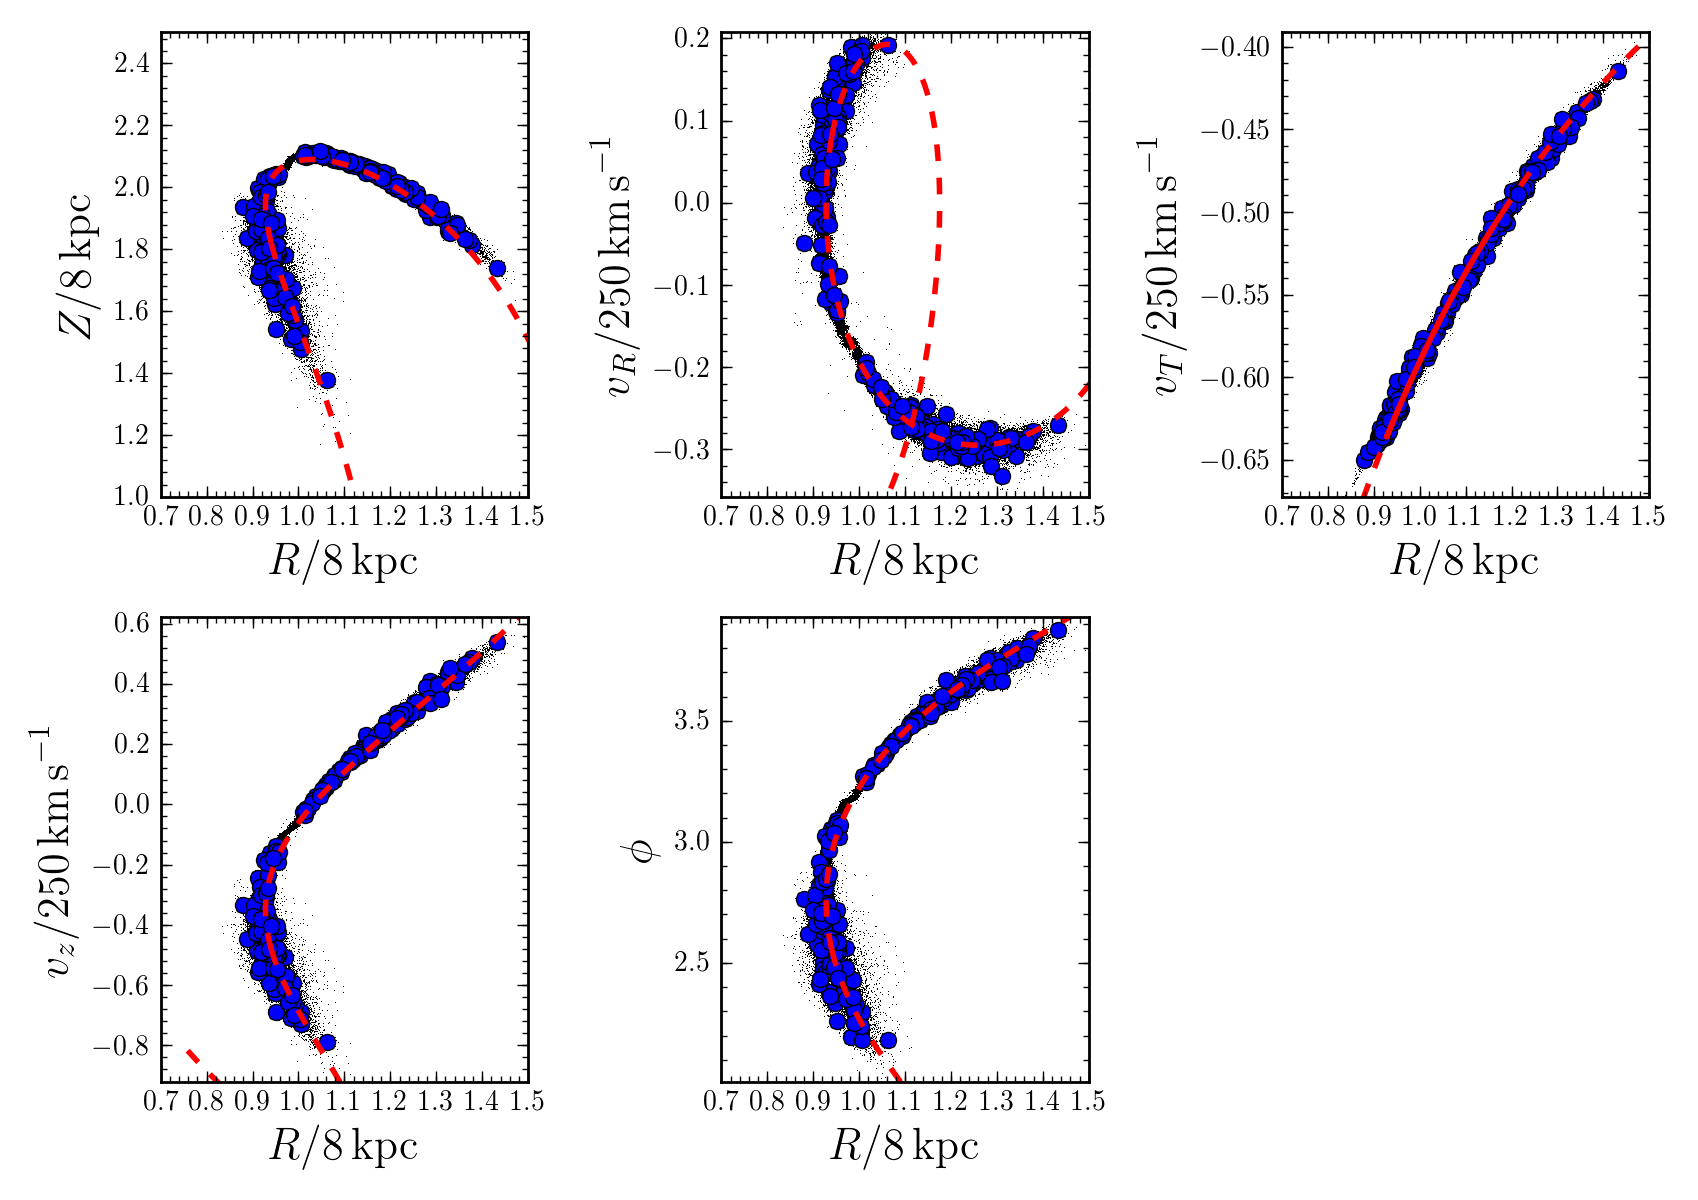
\includegraphics[width=83mm]{./figures/jo_orbitfit.png}
  \caption{Jo's results (Sec.~\ref{ssec:jo_results})}
  \label{plot_jo_orbitfit}
\end{figure}

I computed the acceleration at Pal 5 and get
$a(Pal5) = 3.42 \pm 0.04 pc/Myr^2$.

The PDF in Fig.~\ref{plot_jo_results} shows 1, 2, and 3 sigma contours. 
I just fit a flattened logarithmic potential, so the PDF is for those two parameters ($v_c$ and flattening $q$). 
The orbit fit in Fig.~\ref{plot_jo_orbitfit} shows different projections: I fit to the 200 blue points, the best-fitting orbit is shown in red.


\subsection{Adrian Price-Whelan}\label{ssec:adrian_results}
\begin{figure}
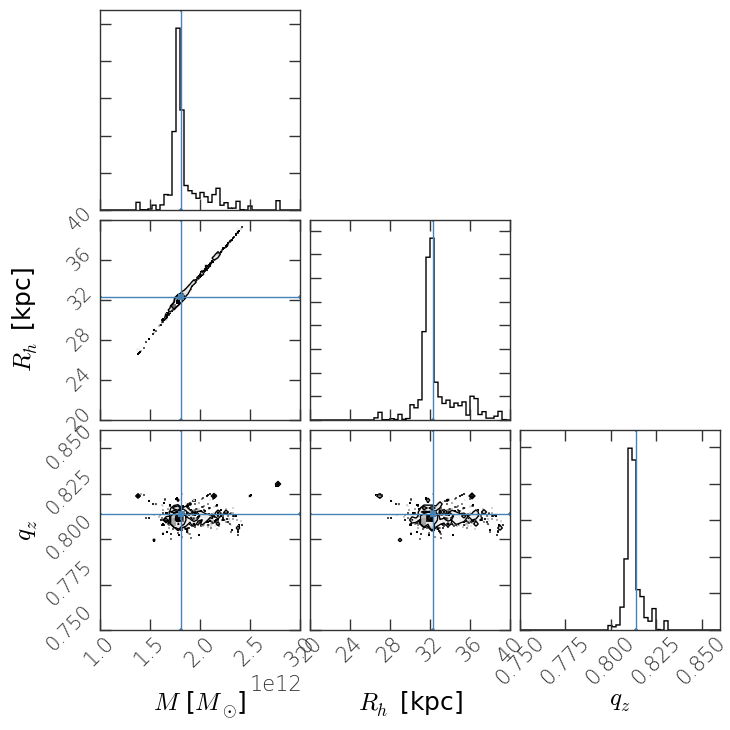
\includegraphics[width=83mm]{figures/adrian_results.png}
  \caption{Adrian's results (Sec.~\ref{ssec:adrian_results})}
  \label{plot_adrian_results}
\end{figure}
\begin{figure}
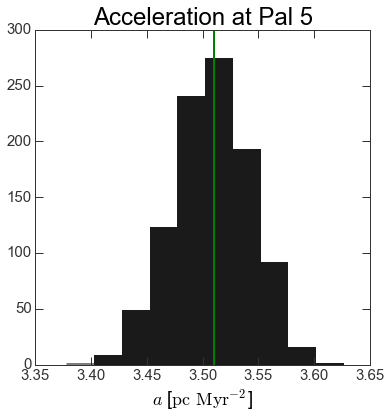
\includegraphics[width=83mm]{figures/adrian_acc.png}
  \caption{Adrian's results (Sec.~\ref{ssec:adrian_results})}
  \label{plot_adrian_acc}
\end{figure}

Adrian's results in Fig.~\ref{plot_adrian_results}. Accelerations in Fig.~\ref{plot_adrian_acc}



\subsection{Jason Sanders}\label{ssec:jason_results}
\begin{figure}
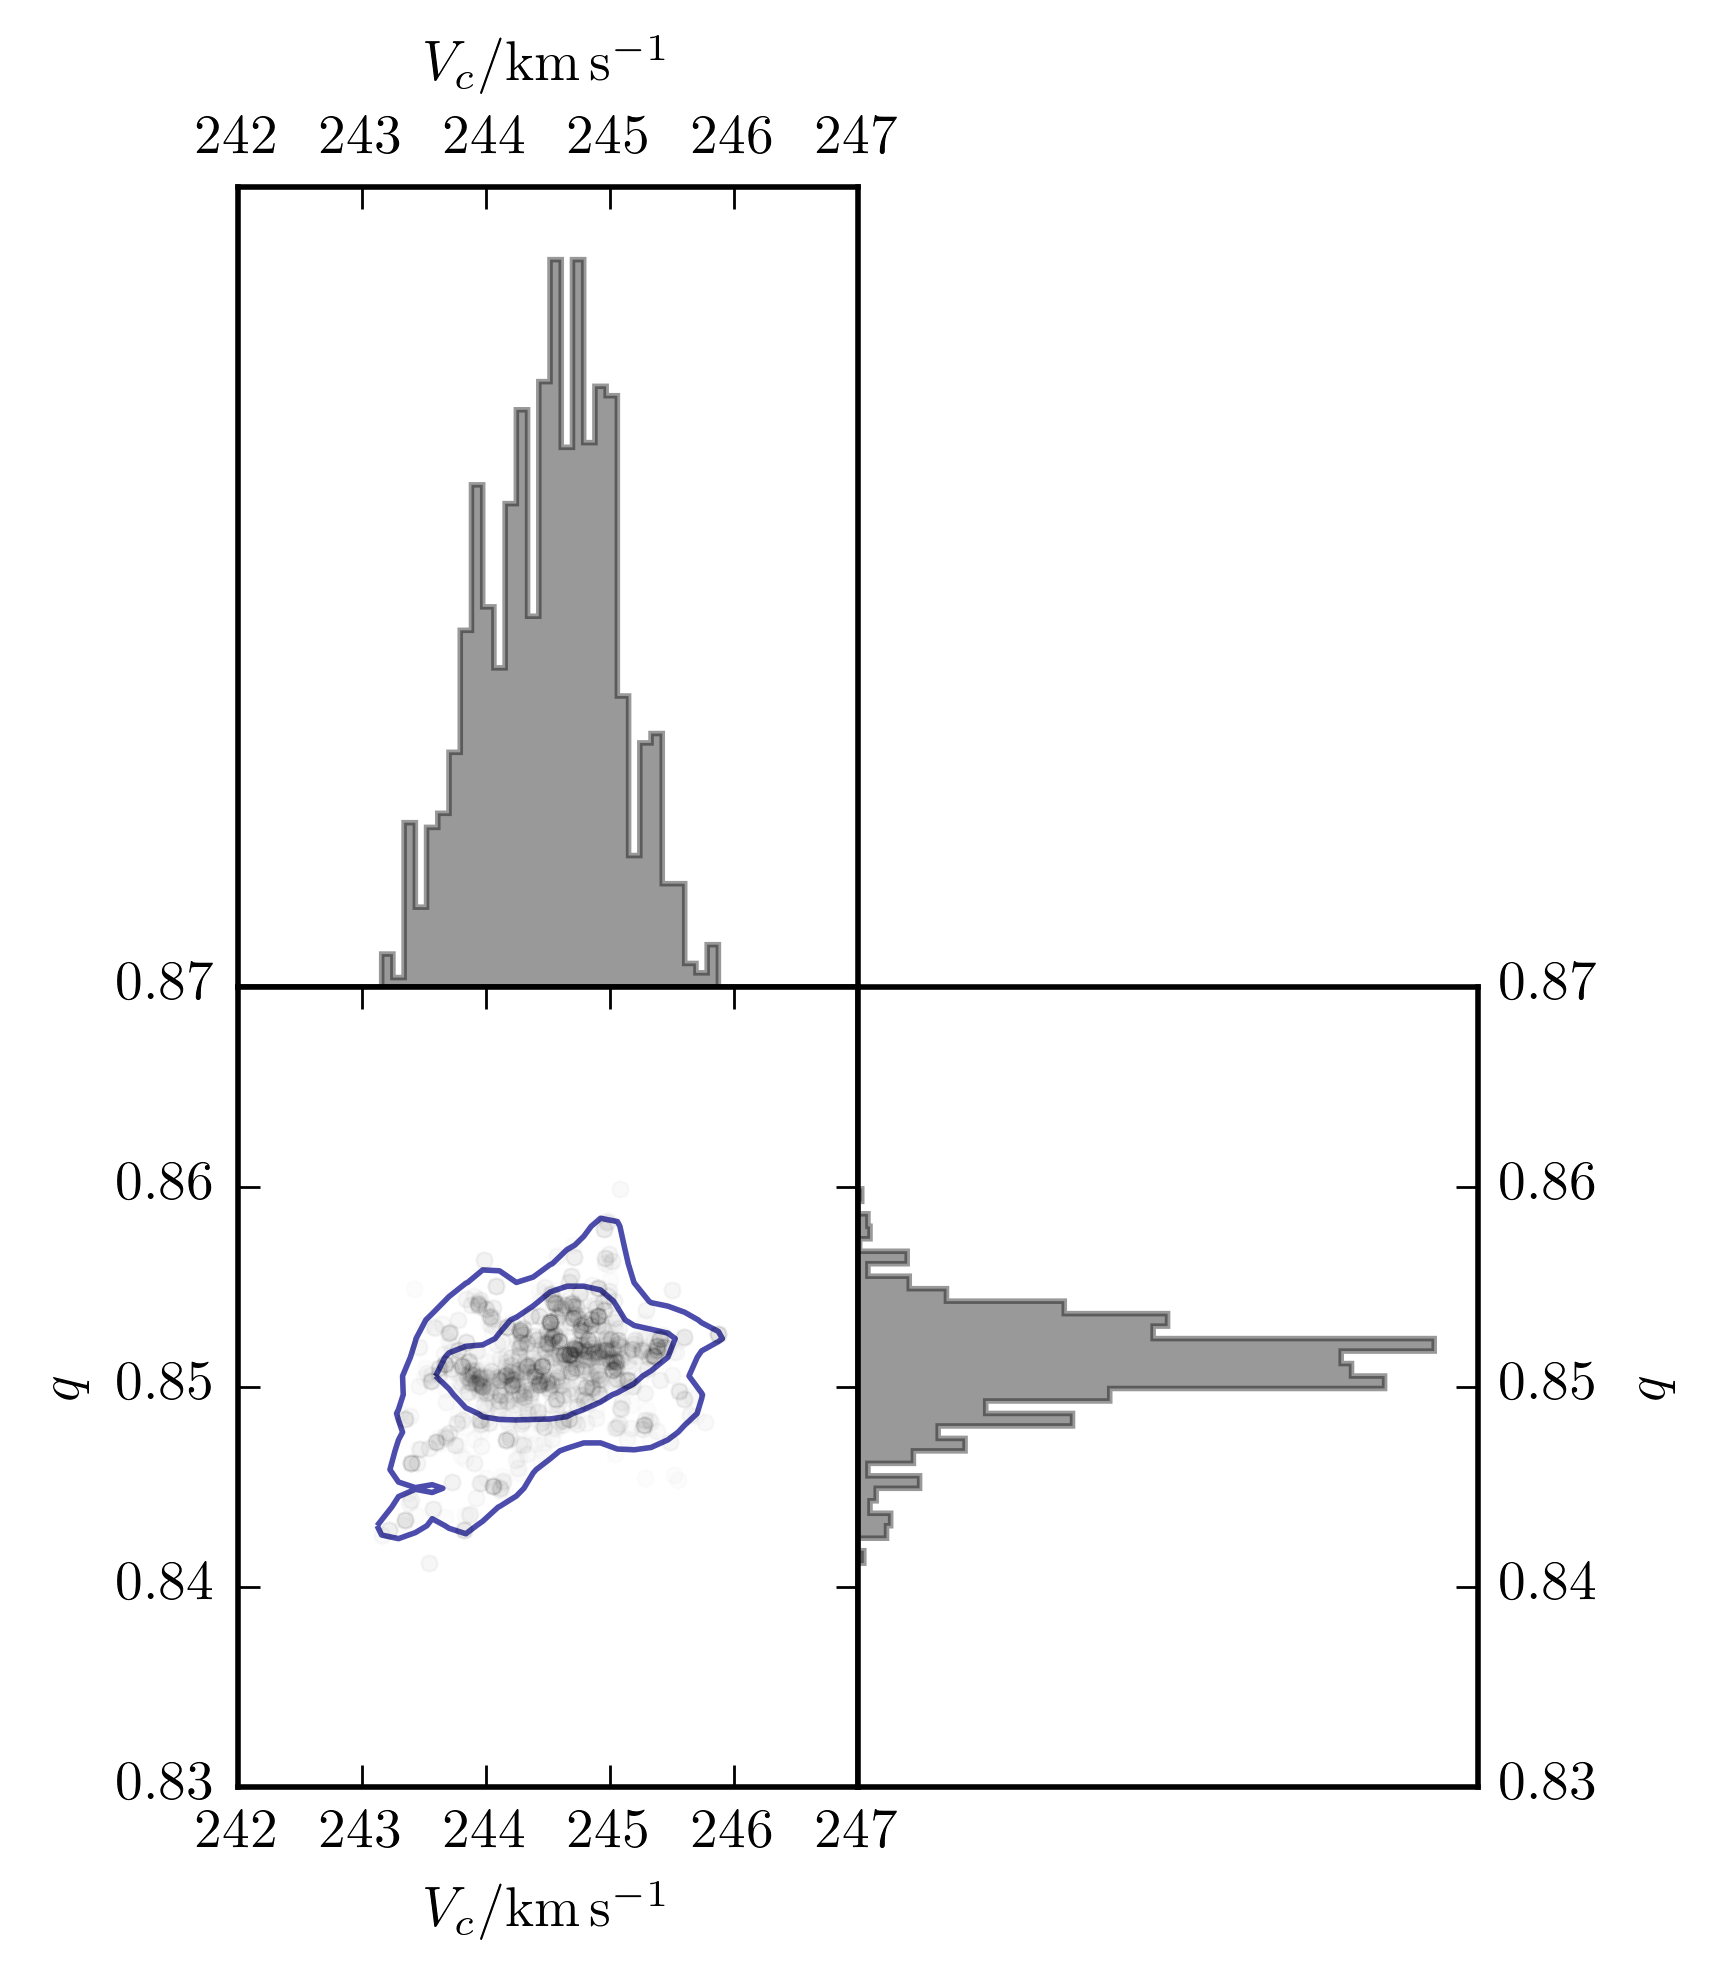
\includegraphics[width=83mm]{./figures/jason_results_logarithmic.png}
  \caption{Jason's results (Sec.~\ref{ssec:jason_results})}
  \label{plot_jason_results_logarithmic}
\end{figure}

\begin{figure}
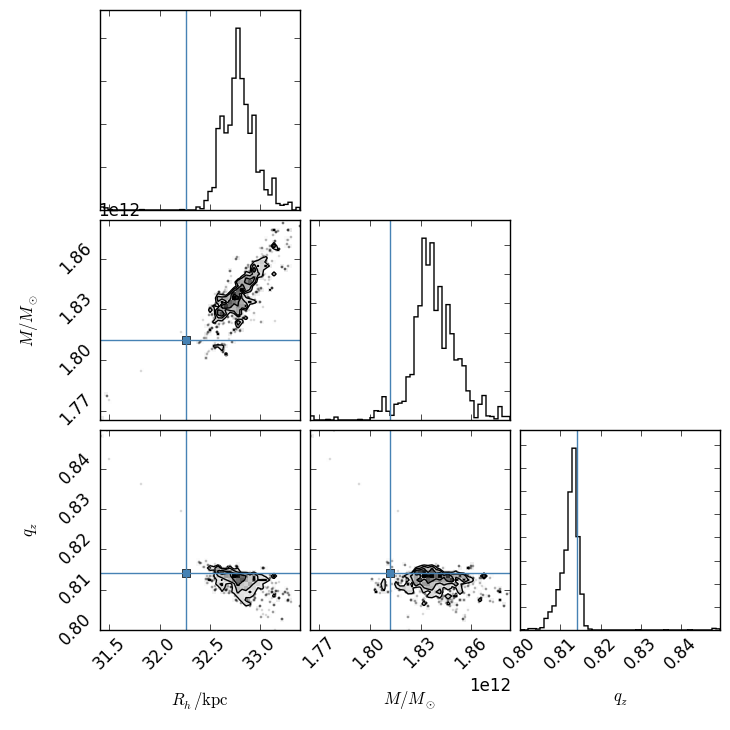
\includegraphics[width=83mm]{./figures/jason_results_truepot.png}
  \caption{Jason's results (Sec.~\ref{ssec:jason_results})}
  \label{plot_jason_results_truepot}
\end{figure}

\begin{figure}
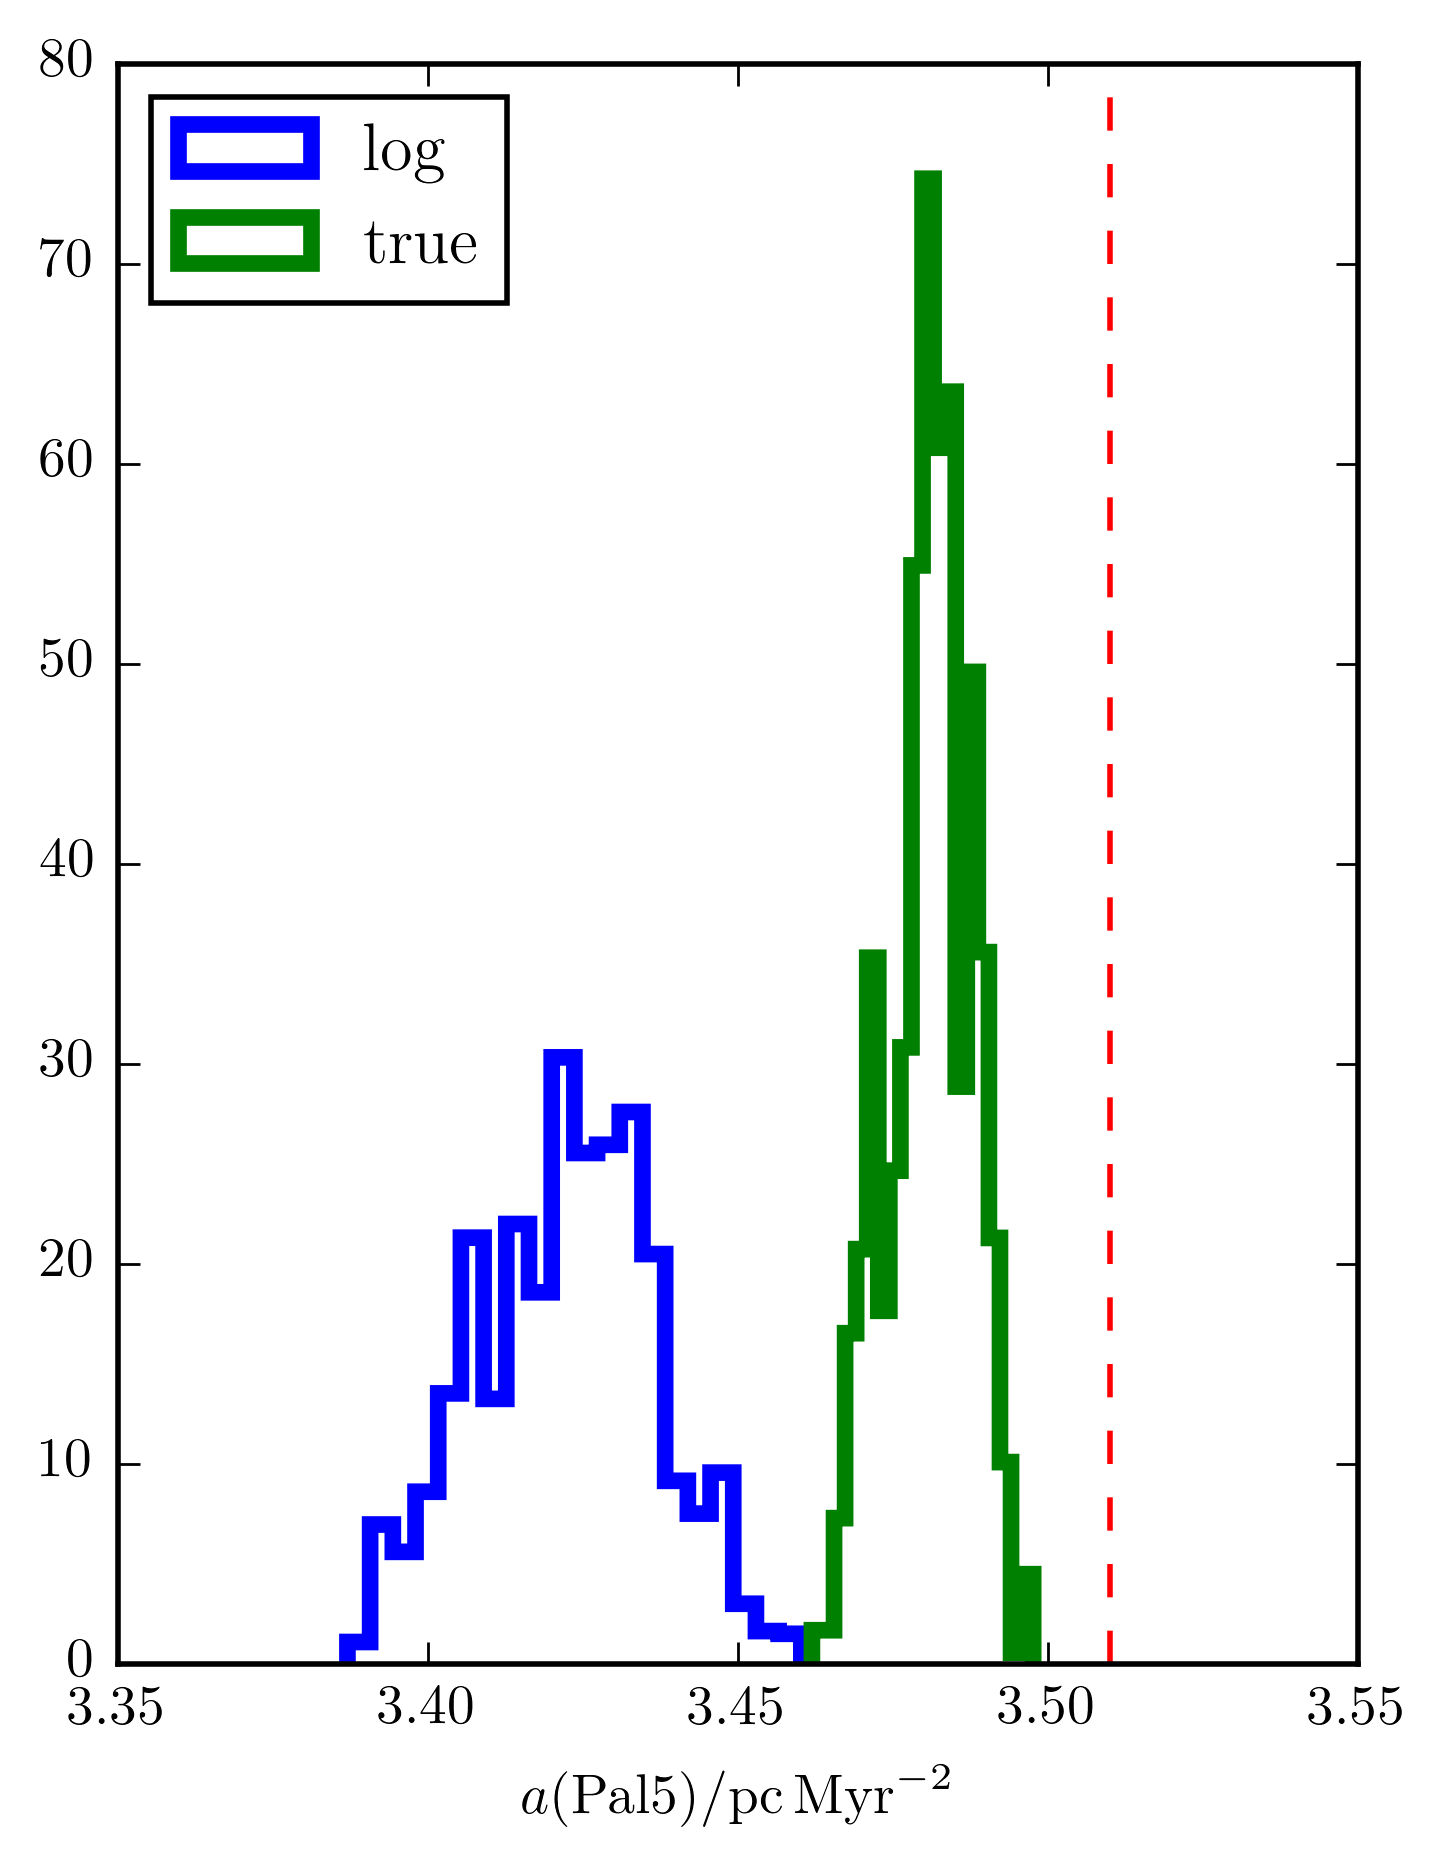
\includegraphics[width=83mm]{./figures/jason_acc.png}
  \caption{Jason's results (Sec.~\ref{ssec:jason_results})}
  \label{plot_jason_acc}
\end{figure}

The blue histogram in Fig.~\ref{plot_jason_acc} is the acceleration-at-Pal5 distribution using the logarithmic and green is using the correct potential form. The red line shows the true value.




\section{Conclusions}
\input{conclusions.tex}


\section*{Acknowledgements}
\input{acknowledgements.tex}

\begin{thebibliography}{99}
\bibitem[\protect\citeauthoryear{Aarseth}{2003}]{Aarseth03} 
Aarseth S.~J., 2003, Gravitational N-Body Simulations, Cambridge, UK, Cambridge University Press 

\bibitem[\protect\citeauthoryear{Bonaca et al.}{2014}]{Bonaca14} 
Bonaca A., Geha M., K{\"u}pper A.~H.~W., Diemand J., Johnston K.~V., Hogg D.~W., 2014, ApJ, 795, 94 

\bibitem[\protect\citeauthoryear{Deg \& Widrow}{2013}]{Deg13} 
Deg N., Widrow L., 2013, MNRAS, 428, 912 

\bibitem[\protect\citeauthoryear{Foreman-Mackey et al.}{2013}]{Foreman13} 
Foreman-Mackey D., Hogg D.~W., Lang D., Goodman J., 2013, PASP, 125, 306 

\bibitem[\protect\citeauthoryear{Gillessen et al.}{2009}]{Gillessen09} 
Gillessen S., Eisenhauer F., Trippe S., Alexander T., Genzel R., Martins F., Ott T., 2009, ApJ, 692, 1075 

\bibitem[\protect\citeauthoryear{Harris}{1996}]{Harris96} 
Harris W.~E., 1996, AJ, 112, 1487 

\bibitem[\protect\citeauthoryear{Jaffe}{1983}]{Jaffe83} 
Jaffe W., 1983, MNRAS, 202, 995 

\bibitem[\protect\citeauthoryear{King}{1962}]{King62} 
King I., 1962, AJ, 67, 471 

\bibitem[\protect\citeauthoryear{Koposov, Rix, \& Hogg}{2010}]{Koposov10} 
Koposov S.~E., Rix H.-W., Hogg D.~W., 2010, ApJ, 712, 260 

\bibitem[\protect\citeauthoryear{K{\"u}pper, Lane, \& Heggie}{2012}]{Kupper12} 
K{\"u}pper A.~H.~W., Lane R.~R., Heggie D.~C., 2012, MNRAS, 420, 2700 

\bibitem[\protect\citeauthoryear{K{\"u}pper et al.}{2015}]{Kupper15} 
K{\"u}pper A.~H.~W., Balbinot E., Bonaca A., Johnston K.~V., Hogg D.~W., Kroupa P., Santiago B.~X., 2015, ApJ, 803, 80 

\bibitem[\protect\citeauthoryear{Miyamoto \& Nagai}{1975}]{Miyamoto75} 
Miyamoto M., Nagai R., 1975, PASJ, 27, 533 

\bibitem[\protect\citeauthoryear{Navarro, Frenk, \& White}{1997}]{Navarro97} 
Navarro J.~F., Frenk C.~S., White S.~D.~M., 1997, ApJ, 490, 493 

\bibitem[\protect\citeauthoryear{Nitadori \& Aarseth}{2012}]{Nitadori12} 
Nitadori K., Aarseth S.~J., 2012, MNRAS, 424, 545 

\bibitem[\protect\citeauthoryear{Odenkirchen et al.}{2002}]{Odenkirchen02} 
Odenkirchen M., Grebel E.~K., Dehnen W., Rix H.-W., Cudworth K.~M., 2002, AJ, 124, 1497 

\bibitem[\protect\citeauthoryear{Perryman et al.}{2001}]{Perryman01} 
Perryman M.~A.~C., et al., 2001, A\&A, 369, 339 

\bibitem[\protect\citeauthoryear{Sch{\"o}nrich, Binney, \& Dehnen}{2010}]{Schonrich10} 
Sch{\"o}nrich R., Binney J., Dehnen W., 2010, MNRAS, 403, 1829 


\end{thebibliography}



\bsp \label{lastpage} \end{document}

